\documentclass[border=3pt]{standalone}
\usepackage[T1]{fontenc}
\usepackage[utf8]{inputenc}
\usepackage{lmodern}
\usepackage{amsmath,amssymb}
\usepackage{xcolor}
\usepackage{tikz}
\usepackage{fontawesome5}
\usepackage{ragged2e}
\usetikzlibrary{shapes,shapes.geometric,shapes.misc,arrows.meta,positioning,
                calc,fit,backgrounds,decorations.pathreplacing,
                decorations.markings,patterns,chains}
\usetikzlibrary{decorations.pathreplacing,decorations.markings}
\definecolor{primary}{HTML}{1A5276}
\definecolor{secondary}{HTML}{2E86C1}
\definecolor{accent}{HTML}{E74C3C}
\definecolor{lightbg}{HTML}{EBF5FB}
\definecolor{defbg}{HTML}{FDF2E9}
\definecolor{greenhl}{HTML}{27AE60}
\definecolor{purplehl}{HTML}{8E44AD}
\definecolor{goldhl}{HTML}{B7950B}
\definecolor{tealhl}{HTML}{117A65}
\definecolor{codebg}{HTML}{F4F6F7}
\definecolor{neutral}{HTML}{707B7C}
\definecolor{dom1}{HTML}{1F618D}
\definecolor{dom2}{HTML}{117864}
\definecolor{dom3}{HTML}{6C3483}
\definecolor{dom4}{HTML}{922B21}
\definecolor{dom5}{HTML}{B7950B}
% --- carried over from ccna.sty so figures match the book exactly
\tikzset{
  dev/.style={rounded corners=3pt, draw=#1, fill=#1!8, text=#1!45!black,
              line width=0.9pt, minimum width=1.45cm, minimum height=1.05cm,
              align=center, font=\scriptsize\bfseries, inner sep=2pt},
  wirestyle/.style={line width=0.9pt, neutral!75},
  xconn/.style={line width=0.9pt, neutral!75, dash pattern=on 2.5pt off 2pt},
}

\newcommand{\Rtr}[3]{\node[dev=dom3] (#1) at #2 {\faIcon{route}\\#3};}
\newcommand{\Sw}[3]{\node[dev=dom2] (#1) at #2 {\faIcon{sitemap}\\#3};}
\newcommand{\Msw}[3]{\node[dev=dom3] (#1) at #2 {\faIcon{layer-group}\\#3};}
\newcommand{\Host}[3]{\node[dev=neutral] (#1) at #2 {\faIcon{desktop}\\#3};}
\newcommand{\Lap}[3]{\node[dev=neutral] (#1) at #2 {\faIcon{laptop}\\#3};}
\newcommand{\Srv}[3]{\node[dev=dom1] (#1) at #2 {\faIcon{server}\\#3};}
\newcommand{\Ap}[3]{\node[dev=dom5] (#1) at #2 {\faIcon{wifi}\\#3};}
\newcommand{\Wlc}[3]{\node[dev=dom5] (#1) at #2 {\faIcon{broadcast-tower}\\#3};}
\newcommand{\Fw}[3]{\node[dev=dom4] (#1) at #2 {\faIcon{shield-alt}\\#3};}
\newcommand{\Cld}[3]{\node[dev=neutral] (#1) at #2 {\faIcon{cloud}\\#3};}
\newcommand{\Phone}[3]{\node[dev=dom5] (#1) at #2 {\faIcon{phone-alt}\\#3};}
\newcommand{\Prn}[3]{\node[dev=neutral] (#1) at #2 {\faIcon{print}\\#3};}

% A link. The optional argument takes tikz options (e.g. xconn for a
% trunk drawn dashed); the fourth argument labels the link.
\newcommand{\wire}[4][wirestyle]{%
  \draw[#1] (#2) -- node[font=\tiny, text=neutral!85!black, fill=white,
                          inner sep=1.2pt, midway] {#4} (#3);}
\newcommand{\plainwire}[3][wirestyle]{\draw[#1] (#2) -- (#3);}


\newenvironment{topology}[1][]
  {\begin{center}\begin{tikzpicture}[font=\scriptsize,#1]}
  {\end{tikzpicture}\end{center}}


\newcommand{\cmd}[1]{\texttt{\small #1}}
\newcommand{\term}[1]{\textbf{\textcolor{primary}{#1}}}
\newcommand{\chref}[1]{Chapter~\ref{ch:#1}}
\newcommand{\ccnafitw}[1]{#1}
\providecommand{\thefigure}{}
% --- progressive builds
\newcount\buildlevel \buildlevel=99
% \stepvis{n}{..} appears from level n onward; \steponly{n}{..} at
% level n alone, which is how a caption is swapped rather than
% accumulated as the build advances. \stepdim{n}{..} is the
% complement of \stepvis: it shows only BEFORE level n, so a
% pair of them draws an element faint and then solid. That keeps
% the canvas full from step 1, which matters for a figure whose
% shape is itself the lesson -- a five-rung ladder revealed one
% rung at a time leaves a void where the method should be.
\newcommand{\stepvis}[2]{\ifnum#1>\buildlevel\relax\else#2\fi}
\newcommand{\steponly}[2]{\ifnum#1=\buildlevel #2\fi}
\newcommand{\stepdim}[2]{\ifnum#1>\buildlevel #2\fi}
% Slide text does not hyphenate. A projected caption broken as
% ``uni-cast'' costs the reader a beat that print can afford and a
% lecture cannot, and the ragged edge it avoids is invisible at
% four metres anyway.
\hyphenpenalty=10000 \exhyphenpenalty=10000
\begin{document}
\buildlevel=2
% Slide build of Figure 3.1 -- deliberately NOT the book's layout.
%
% In print the book shows two panels side by side, because a reader compares
% them at a glance. On a slide that wastes two thirds of the canvas at step 1
% and makes the first thing the room sees the smallest. Here the same story is
% told by ONE diagram that evolves in place:
%
%   1  a frame arrives from PC-A and the switch does not know the destination
%   2  so it floods it everywhere except back the way it came
%   3  the reply teaches the switch, and the table now holds PC-D
%
% \stepvis{n}{...} shows from level n onward; \steponly{n}{...} at level n
% alone, which is how the caption is swapped rather than accumulated.
\begin{tikzpicture}[font=\scriptsize]
  \tikzset{
    dv/.style={rounded corners=3pt, draw=#1, fill=#1!8, text=#1!45!black,
               line width=0.9pt, minimum width=1.45cm, minimum height=1.05cm,
               align=center, font=\scriptsize\bfseries},
    fl/.style={-{Stealth[length=2.6mm]}, line width=1.4pt}}

  % Fixed canvas: identical at every level so Morph fades rather than slides.
  % \useasboundingbox, not \path -- a path only ever grows the box, so the
  % step with the widest caption came out a different size and Morph then
  % slid the whole diagram sideways instead of fading parts into it.
  \useasboundingbox (-1.9,-2.7) rectangle (11.3,2.3);

  \node[dv=dom2, minimum width=7.4cm] (sw) at (3.0,1.15) {\faIcon{sitemap}\\SW1};
  \foreach \x/\n in {0.6/A, 2.2/B, 3.8/C, 5.4/D}
    \node[dv=neutral] at (\x,-0.9) {\faIcon{desktop}\\PC-\n};

  % the frame arriving -- present at every level
  \draw[fl, dom2!85] (0.6,-0.35) -- (0.6,0.6);
  \node[font=\scriptsize, text=dom2!45!black, anchor=east] at (0.4,0.15) {in};

  \stepvis{2}{\foreach \x in {2.2, 3.8, 5.4}
      \draw[fl, accent!80] (\x,0.6) -- (\x,-0.35);}

  \stepvis{3}{%
    \node[draw=neutral!55, fill=codebg, rounded corners=3pt, line width=0.8pt,
          font=\scriptsize\ttfamily, align=left, inner sep=6pt]
        at (8.4,1.15)
        {MAC address table\\[3pt]
         \textcolor{neutral!70!black}{aaaa.aaaa.aaaa~~Gi0/1}\\
         \textcolor{accent!70!black}{dddd.dddd.dddd~~Gi0/4}};
    \draw[dom2!45, line width=0.8pt, dash pattern=on 2.5pt off 2pt]
        (5.4,-0.35) -- (7.4,0.75);}

  \steponly{1}{\node[font=\bfseries, text=neutral!45!black, anchor=north west]
      at (-1.6,-1.75) {Destination not in the table. Now what?};}
  \steponly{2}{\node[font=\bfseries, text=accent!75!black, anchor=north west]
      at (-1.6,-1.75)
      {Flood: every port in the VLAN except the one it arrived on};}
  \steponly{3}{\node[font=\bfseries, text=dom2!50!black, anchor=north west]
      at (-1.6,-1.75)
      {PC-D replies --- and the switch has now learned where it is};}
\end{tikzpicture}

\end{document}
